% !TeX root = ../main.tex

\chapter{引言}
\label{chap:intro}

基于闪存的固态硬盘(SSD)正在数据中心中得到越来越广泛的应用。
与机械硬盘(HDD)相比,SSD的吞吐和访问延迟都有数量级的提升~\cite{chen2009understanding}。
特别地,由于内部存储介质不同,SSD的随机访问性能尤为出色。
因此,主流的云计算厂商,如Azure、AWS等,都提供了基于SSD的高性能存储服务~\cite{awsebs,azuredisks}。
专门针对固态硬盘进行优化的键值存储引擎RocksDB也得到了广泛的部署~\cite{cao2020characterizing,rocksdb,siying2021rocksdb}。

与此同时,为了解决数据中心资源利用率低的问题~\cite{kanev2015profiling},研究人员提出了资源池化(Resource Disaggregation)的方法~\cite{shan2018legoos,klimovic2016flash}。
通过将原本紧耦合的CPU、内存、硬盘等资源分别组织成独立的资源池,云服务商可以调度多租户共用物理资源,使有限的资源得到尽可能大的复用,避免浪费。
因此,资源池化在学术界和工业界都受到了广泛的关注。
目前,资源池化已经广泛地存在于云存储服务中。
Azure Blob Storage~\cite{azureblob}、AWS S3~\cite{awss3}等对象存储服务
和Azure Disk Storage~\cite{azuredisks}、AWS Elastic Block Store~\cite{awsebs}等块存储服务
都提供了独立于计算服务的、多租户共享的存储抽象。

然而,SSD等高速设备的出现给存储资源池化带来了新的挑战——多租户间的性能隔离。
当多个租户共享同一块物理硬盘时,他们的访问性能不应相互影响。
这一保证在SSD上不易实现。
由于基于闪存的SSD的内在特性,共享同一块物理SSD的多个租户之一进行的写操作可能会触发SSD的垃圾回收、缓冲区清除等内部维护行为,这些行为将会影响其它租户的访问性能。
特别地,这一读写干扰~\cite{klimovic2017reflex}问题会使其它租户的访问尾延迟增加数倍。
对于追求快速响应的Web服务而言,这意味着其服务质量将受到较大的影响~\cite{dean2013tail}。
因此,追求低延迟的应用仍倾向于使用本地独占的SSD存储~\cite{awsvm,azurevm}。

\begin{figure}[h]
  \centering
  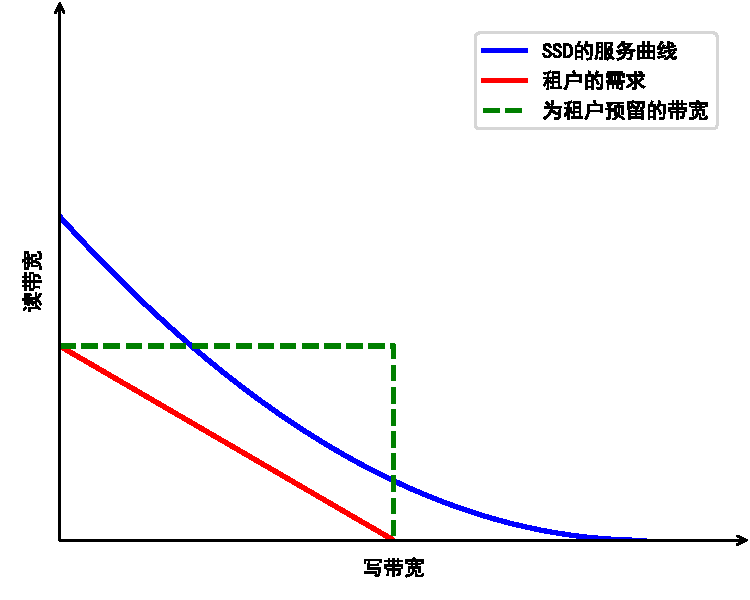
\includegraphics[width=0.6\textwidth]{thesis-intro-cmp.pdf}
  \caption{
        由于SSD读写操作的不对称性,简单的限制读写带宽会造成资源的浪费。
      }
  \label{fig:intro}
\end{figure}

简单限制各个租户分享到的最大带宽的方式不能保证各个租户的访问尾延迟,因此不能实现性能隔离。
并且,由于SSD的读写操作对磁盘的影响并不对称,需要为读和写分别设置最大带宽,但租户往往不会同时达到读和写的最大带宽,这会造成SSD带宽的浪费。
因此,本文使用\textit{SLA曲线}(Service Level Agreement)来描述服务质量。
具体来讲,SLA曲线表示的是在某个尾延迟要求下的最大读写带宽。
硬盘在保证尾延迟下的最大可达带宽可以用SLA曲线描述。
例如,\JF{加图:PM963}。
应用对于服务质量的需求也可以用SLA曲线描述。
例如,\JF{加图:RocksDB}。

针对以上问题,本研究搭建了一个具有多租户性能隔离功能的SSD资源池化存储系统,该系统具有如下设计目标:
\textbf{1)高资源利用率}。
通过资源池化,资源调度不再受限于“服务器”这一有限的单位。
本系统可以调度多租户共享同一物理硬盘上的存储空间和带宽,达到资源的高效利用;
\textbf{2)用户自定义SLA}。
在资源池化的系统中,用户对存储资源的需求也不再受限于服务器上有限的资源。
本系统允许用户使用\textit{SLA曲线}定义其需要的读写带宽及达到该带宽时的尾延迟,系统会根据该定义为用户自动分配适合的存储硬盘。
\textbf{3)低尾延迟}。
本系统将各租户可保证的尾延迟作为存储性能隔离的评价指标。
通过减少或控制占用同一物理硬盘的各租户间的读写干扰,本系统可以降低各租户的尾延迟,从而实现有效的存储性能隔离。
\autoref{tab:cmp-ebs-insstore}中为本系统与目前主流云存储系统的对比。

\begin{table}[h]
  \centering
  \caption{本系统与常见云存储系统的对比}
  \label{tab:cmp-ebs-insstore}
  \begin{tabular}{cccc}
    \toprule
    \textbf{} & 高资源利用率 & 自定义SLA & 低尾延迟  \\
    \midrule
    传统池化存储系统 & \cmark & 部分 & \xmark  \\
    直连的闪存系统 & \xmark & \xmark & \cmark   \\
    \textbf{本系统} & \cmark & \cmark & \cmark  \\
    \bottomrule
  \end{tabular}
\end{table}

为了实现以上设计目标,本系统进行了如下设计。
首先,为了改善多租户读写干扰问题,本系统设计了无读写干扰的SSD阵列。
本系统提出\textit{分离的读写时间窗口},将对SSD的读写混合访问拆分为交替的纯读和批量写访问。
在纯读时间窗口中,本系统将所有写请求存于缓冲区中,从而获得无干扰的读性能;
纯写窗口中批量写入写请求,从而最大程度利用SSD的写带宽。
为了在纯写窗口中仍能服务读请求,本系统通过RAID~\cite{patterson1988case}或纠删码~\cite{huang2012erasure}等方式引入冗余。
通过协调不同硬盘中的时间窗口,使得所有数据总能被以无干扰的延迟被访问。

在此基础上,针对不同用户的不同SLA需求,本系统设计了满足SLA要求的数据分布算法。
本研究认为,现代存储应用的服务质量要求不应单纯以限制最大读写带宽实现。
因此,本研究提出用SLA曲线定义用户的服务质量要求,并由此定义了SLA曲线的加法与减法操作。
基于SLA曲线这一定义,本系统提出了一个多租户、多SSD数据分布的在线启发式算法。
该算法受向量装箱问题~\cite{panigrahy2011heuristics,hu2003operations}的启发,采用最佳适应算法,为系统中的租户提供了SLA保障,还得到了高效的资源利用率。

本文的后续章节按如下方式组织:
第二章介绍本研究的动机——闪存资源池化系统中的多租户性能隔离问题,并介绍在保证SSD的服务质量方面的相关工作;
第三章介绍本研究所提出的系统设计,并详细介绍如何构建无读写干扰的冗余SSD阵列,以及基于背包问题的用户需求分配算法;
第四章介绍该系统的实现方式;
第五章通过大量实验证明了该系统的有效性;
第六章为本研究的总结。